\section{Résultats et Discussions}

\subsection{Évaluation de l'impact de la NAO sur l'upwelling}
\subsubsection{Analyse générale}
Une analyse globale sur l’ensemble du territoire marocain montre que l’upwelling est principalement localisé dans la zone sud, en particulier le long de la côte atlantique sud. Cependant, il est crucial d'examiner le phénomène à l'échelle nationale pour détecter un éventuel impact des changements climatiques sur cette dynamique, notamment dans les zones traditionnellement moins affectées par l'upwelling.

\begin{figure}[H]
\centering
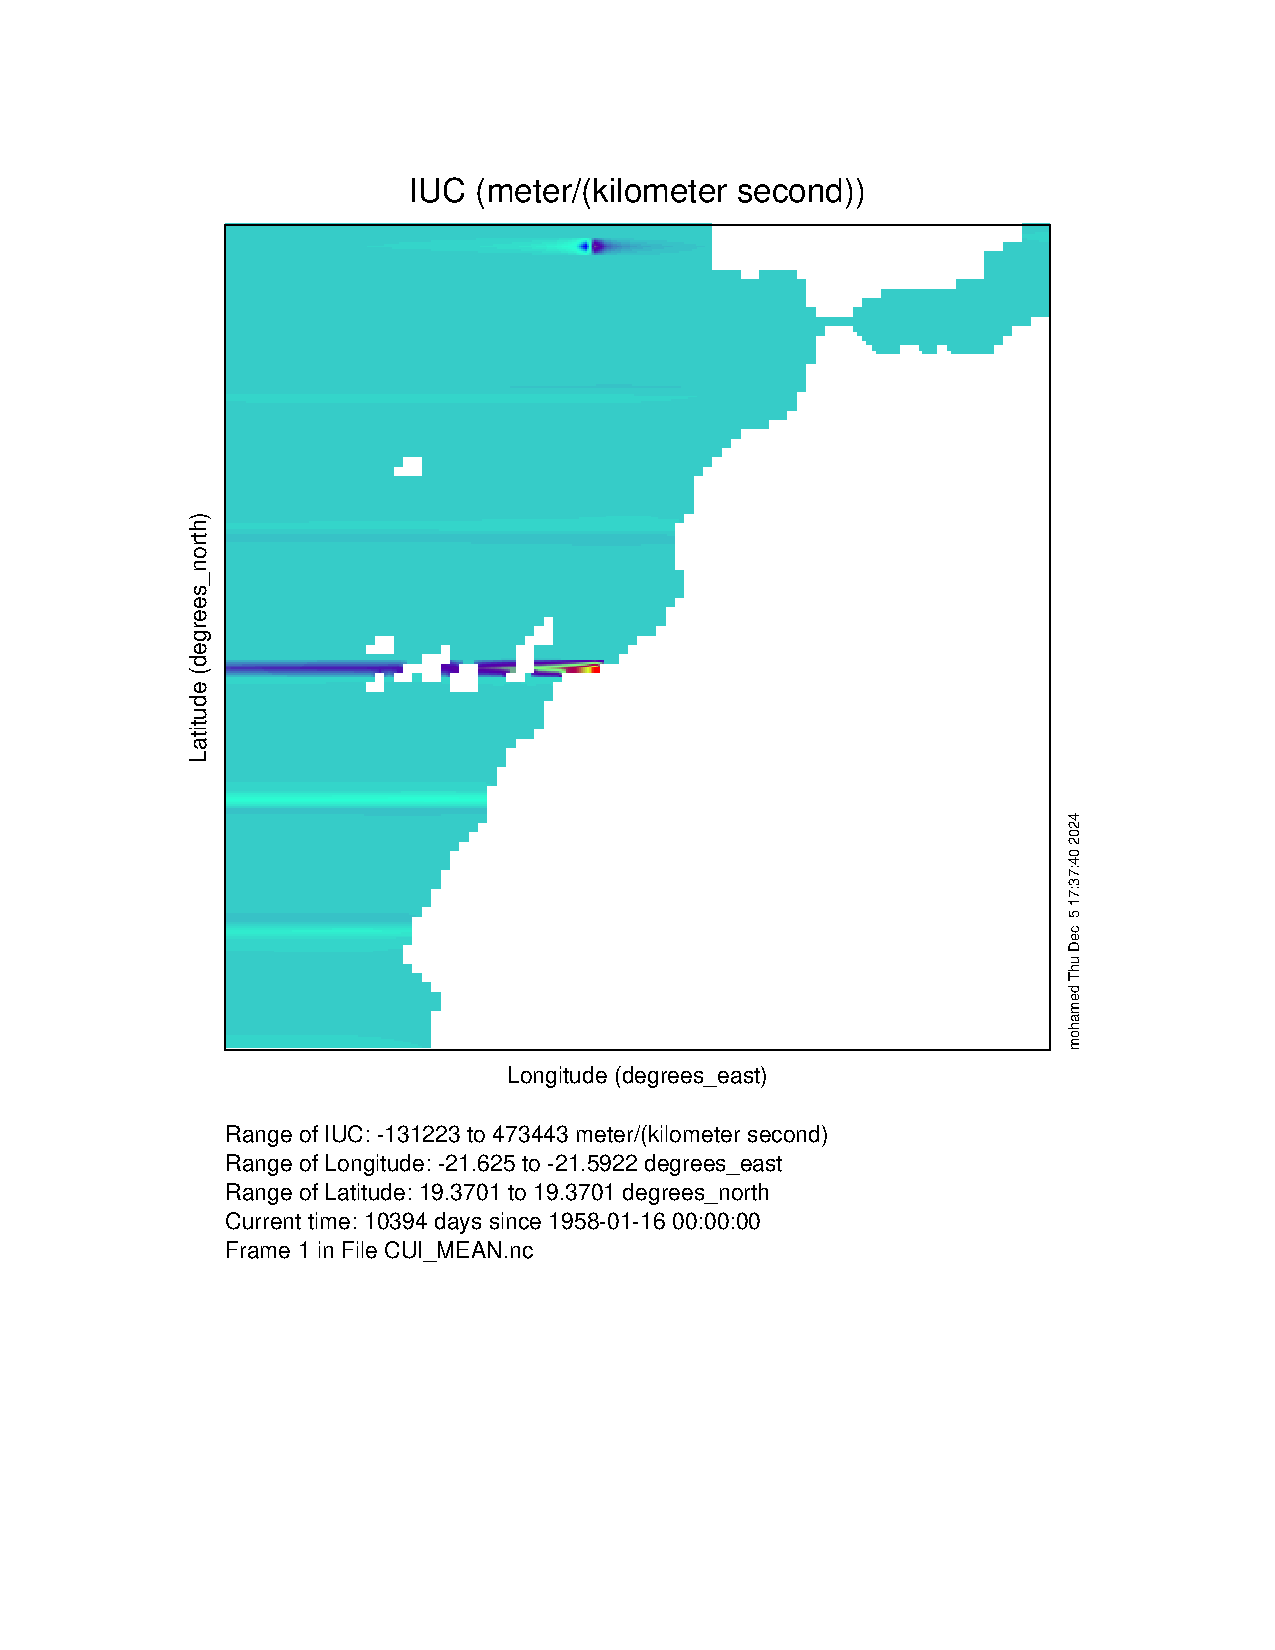
\includegraphics[scale=0.5]{ncview_output.pdf}
\caption{Climatologie de l'upwelling au Maroc (1958–2014).}
\label{fig:climatologie_upwelling}
\end{figure}

La figure~\ref{fig:climatologie_upwelling} montre la répartition spatio-temporelle de l'upwelling au Maroc, confirmant une activité accrue dans la région sud. Ces observations soulignent la nécessité de comprendre les interactions entre les indices climatiques tels que la NAO et les processus océaniques locaux.

\subsubsection{Analyse des distributions}
La figure~\ref{fig:distributions} illustre les distributions de probabilité de l’indice d'upwelling côtier (CUI) et de l'oscillation nord-atlantique (NAO). 

\begin{figure}[H]
\centering
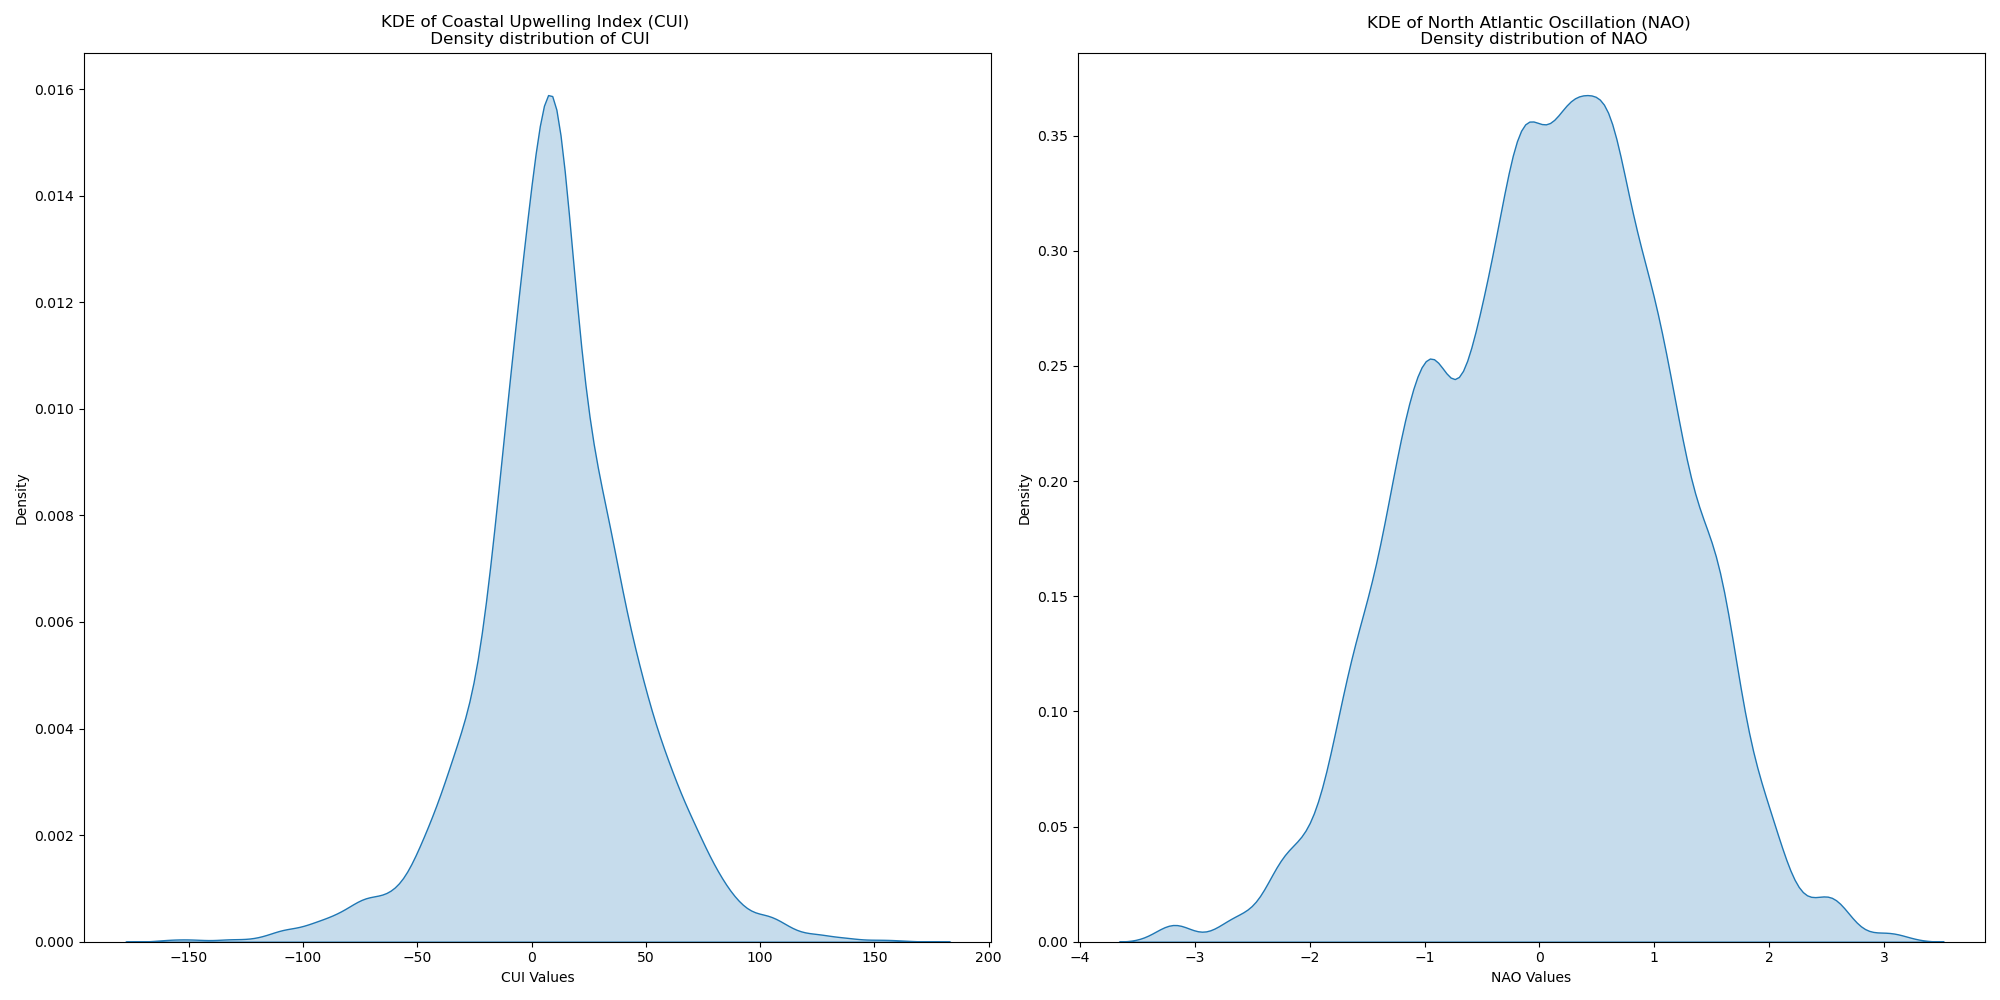
\includegraphics[scale=0.3]{kde_nao_cui.png}
\caption{Distribution de probabilité pour NAO et CUI.}
\label{fig:distributions}
\end{figure}

Les deux indices suivent une distribution normale centrée autour de zéro. Cette symétrie indique que les valeurs extrêmes (positives ou négatives) sont rares, tandis que la majorité des données se concentre autour de la moyenne. Cette caractéristique statistique suggère des variations régulières, bien adaptées pour des analyses de corrélation.

\subsection{Analyse de la corrélation NAO-CUI}
\begin{figure}[H]
\centering
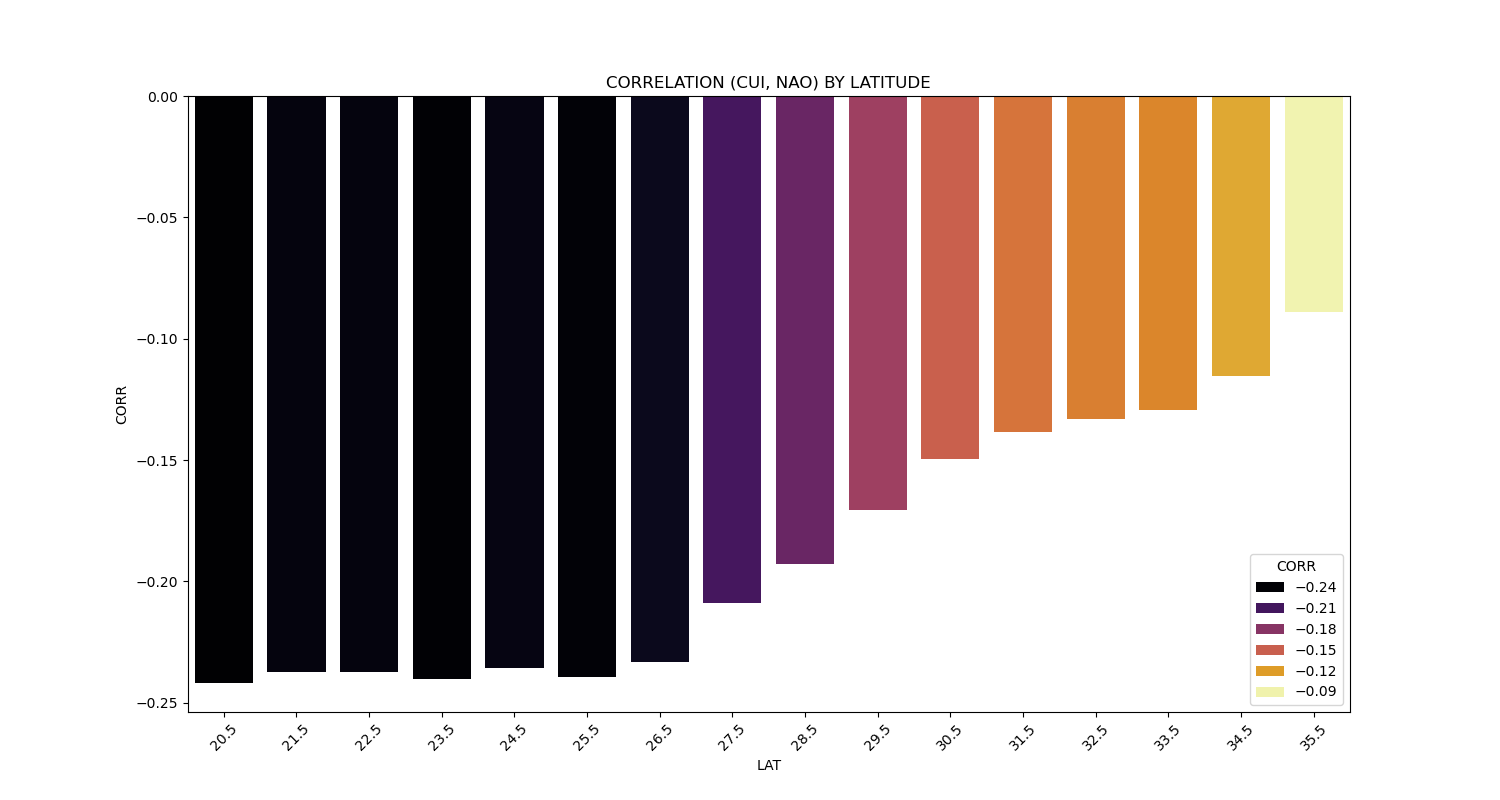
\includegraphics[scale=0.3]{corr.png}
\caption{Corrélation entre la NAO et le CUI en fonction de la latitude.}
\label{fig:correlation}
\end{figure}

La figure~\ref{fig:correlation} met en évidence une corrélation négative entre la NAO et le CUI, avec une intensité qui varie selon la latitude. Les observations principales incluent :
\begin{itemize}
    \item \textbf{Zones méridionales :} La corrélation est fortement négative, indiquant un impact marqué de la NAO sur l'upwelling. Cela correspond aux régions où l’upwelling est historiquement le plus actif, notamment entre Agadir et Lagouira.
    \item \textbf{Zones septentrionales :} La corrélation diminue en intensité, devenant presque nulle. Cela reflète un moindre impact de la NAO sur l’upwelling dans ces régions.
\end{itemize}

Ces résultats corroborent les observations sur le terrain, où les zones sud du Maroc présentent une productivité biologique élevée, stimulée par l'upwelling, ce qui favorise des activités de pêche dynamiques.

\subsection{Impact de la phase de la NAO sur l'upwelling}
Pour explorer davantage l’effet de la NAO, l’analyse a été subdivisée en deux phases distinctes : la phase positive (NAO+) et la phase négative (NAO-). La figure~\ref{fig:impact_phases} illustre les variations du CUI pour chaque phase.

\begin{figure}[H]
\centering
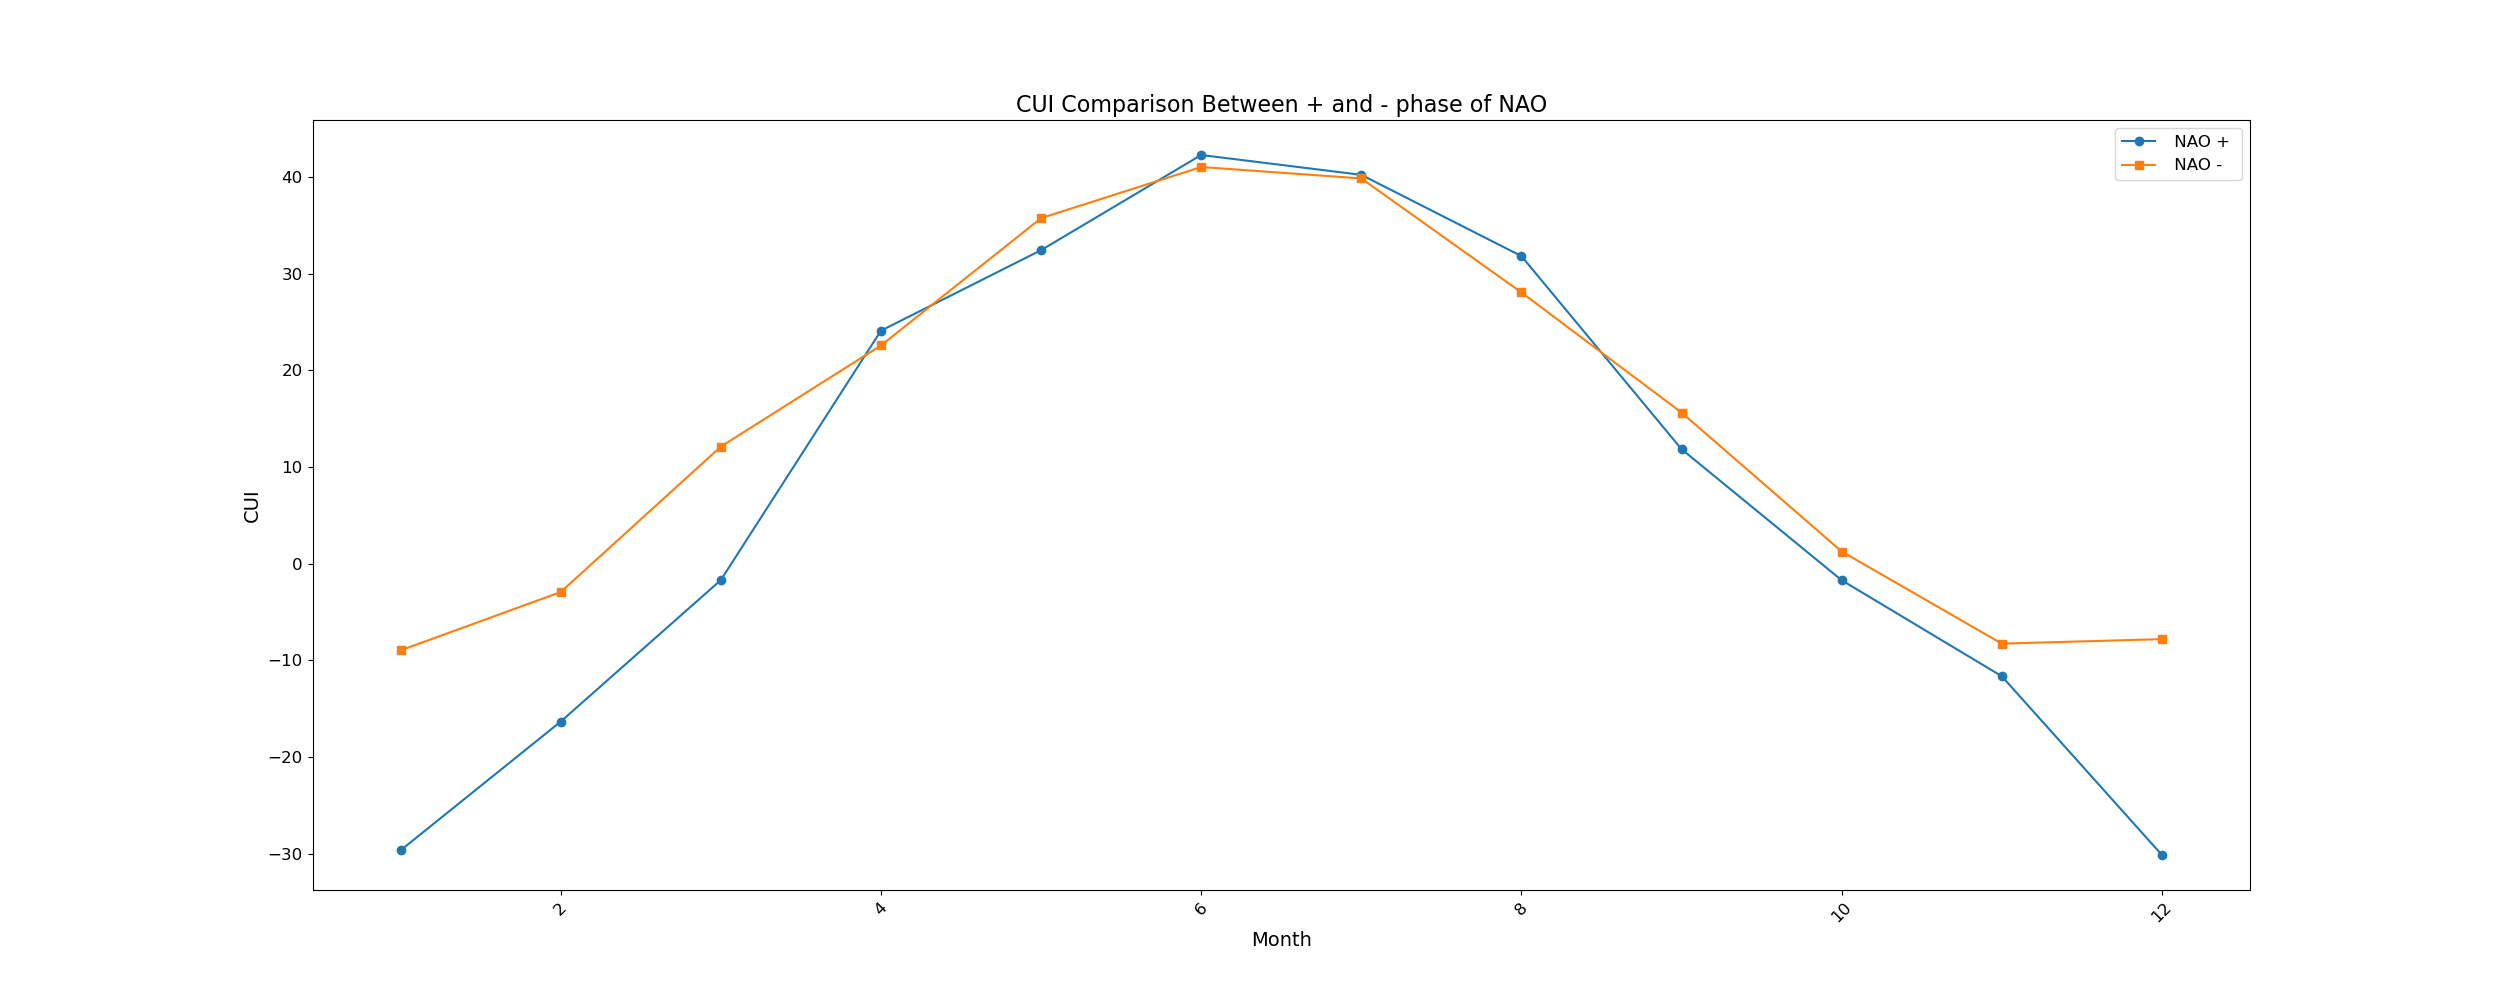
\includegraphics[scale=0.3]{CUI_NAO_PHASES.png}
\caption{Analyse de l'impact des phases de la NAO sur le CUI.}
\label{fig:impact_phases}
\end{figure}

\subsubsection{Phase positive de la NAO (NAO+)}
\begin{figure}[H]
\centering
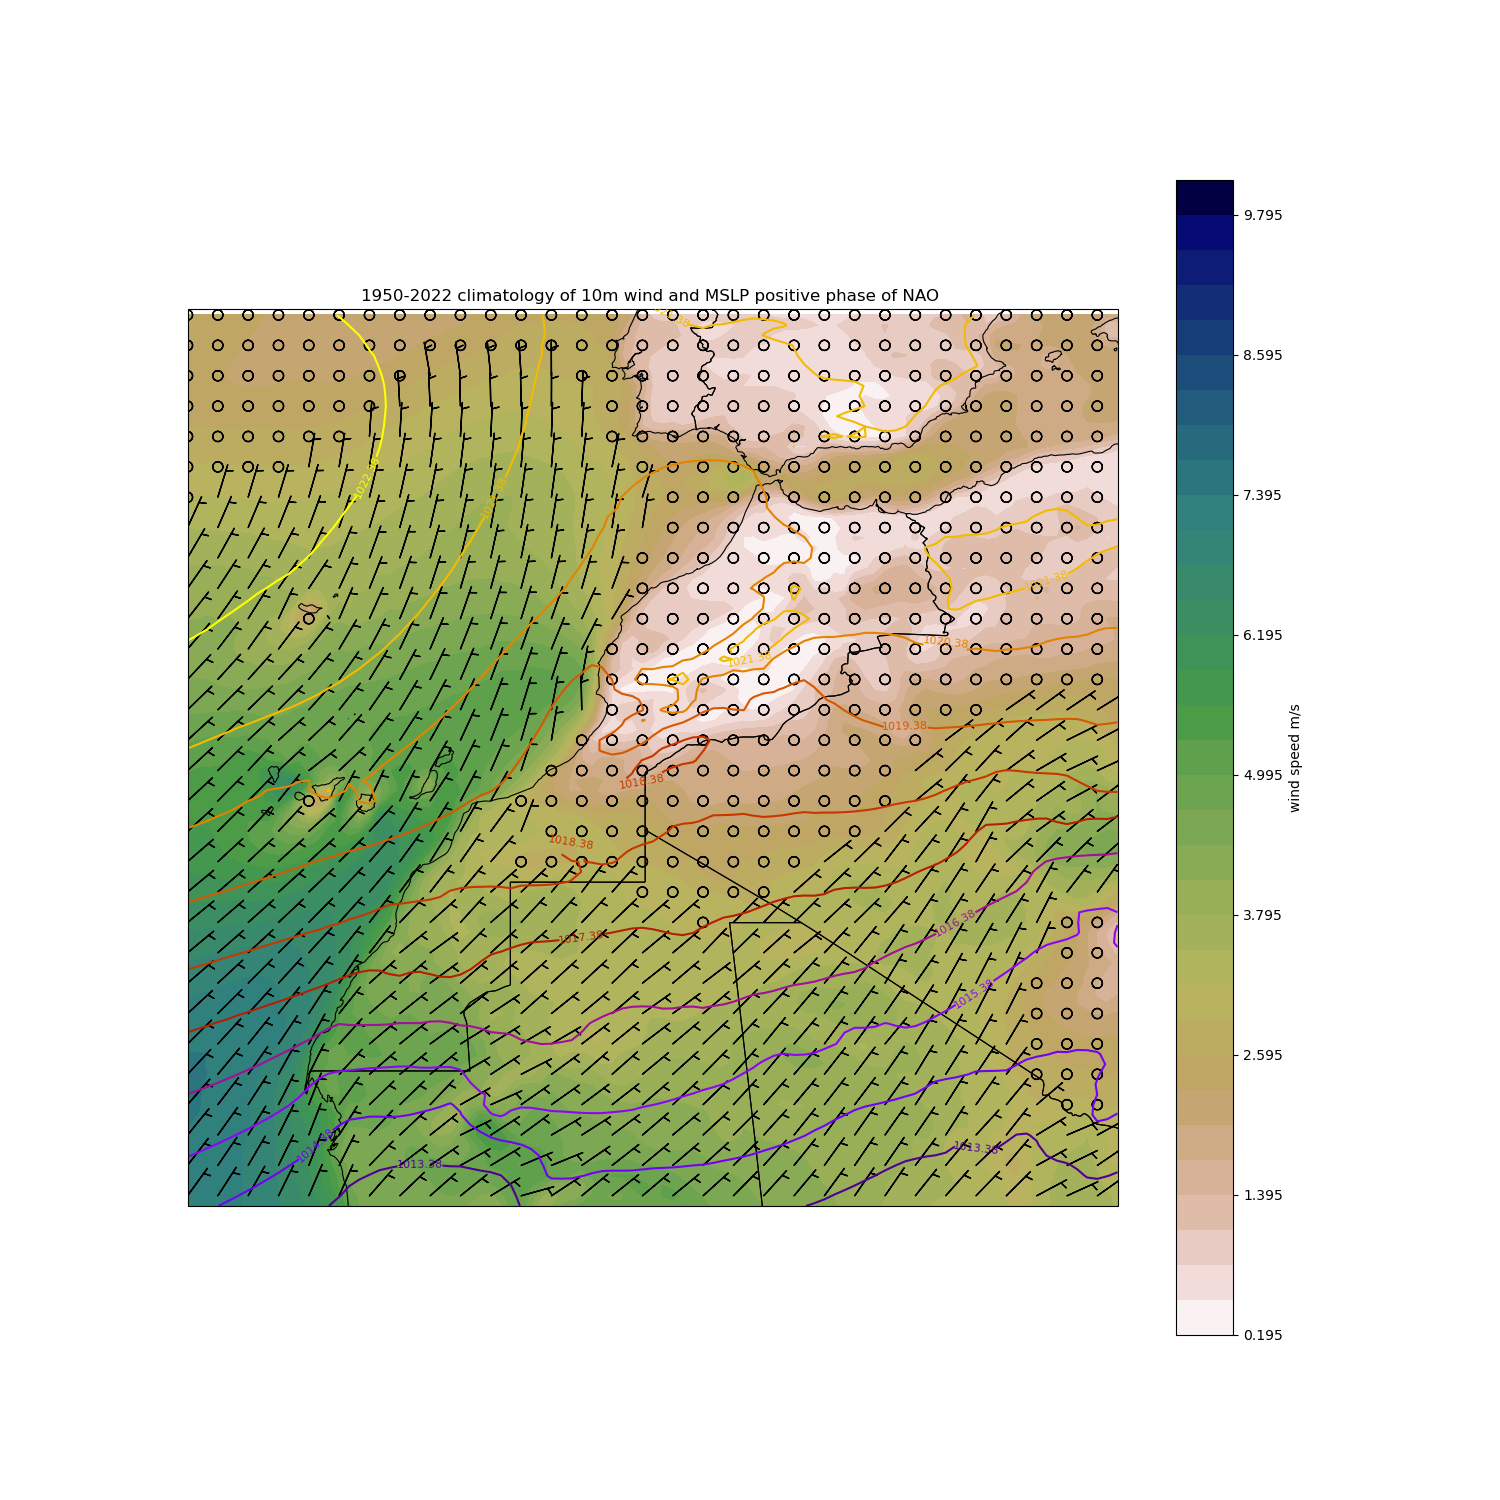
\includegraphics[scale=0.3]{POS_PHASE.png}
\caption{Climatologie du vent et de la pression pour la phase NAO+ (1950–2022).}
\label{fig:nao_positive}
\end{figure}

Lors de la phase NAO+, les caractéristiques atmosphériques et océaniques suivantes sont observées :
\begin{itemize}
    \item \textbf{Direction du vent :} Les vents soufflent moins parallèlement à la côte, réduisant l'efficacité du mécanisme d'upwelling. Cette désorientation est particulièrement visible dans les zones méridionales.
    \item \textbf{Intensité du vent :} La vitesse moyenne du vent ne dépasse pas 3 m/s (environ 6 nœuds), limitant le transport d'Ekman et la remontée des eaux froides riches en nutriments.
    \item \textbf{Impact sur le CUI :} Une phase NAO+ est associée à une diminution significative de l’intensité de l’upwelling, affectant négativement la productivité marine, en particulier dans les zones à forte dépendance économique sur la pêche.
\end{itemize}

\subsubsection{Phase négative de la NAO (NAO-)}
\begin{figure}[H]
\centering
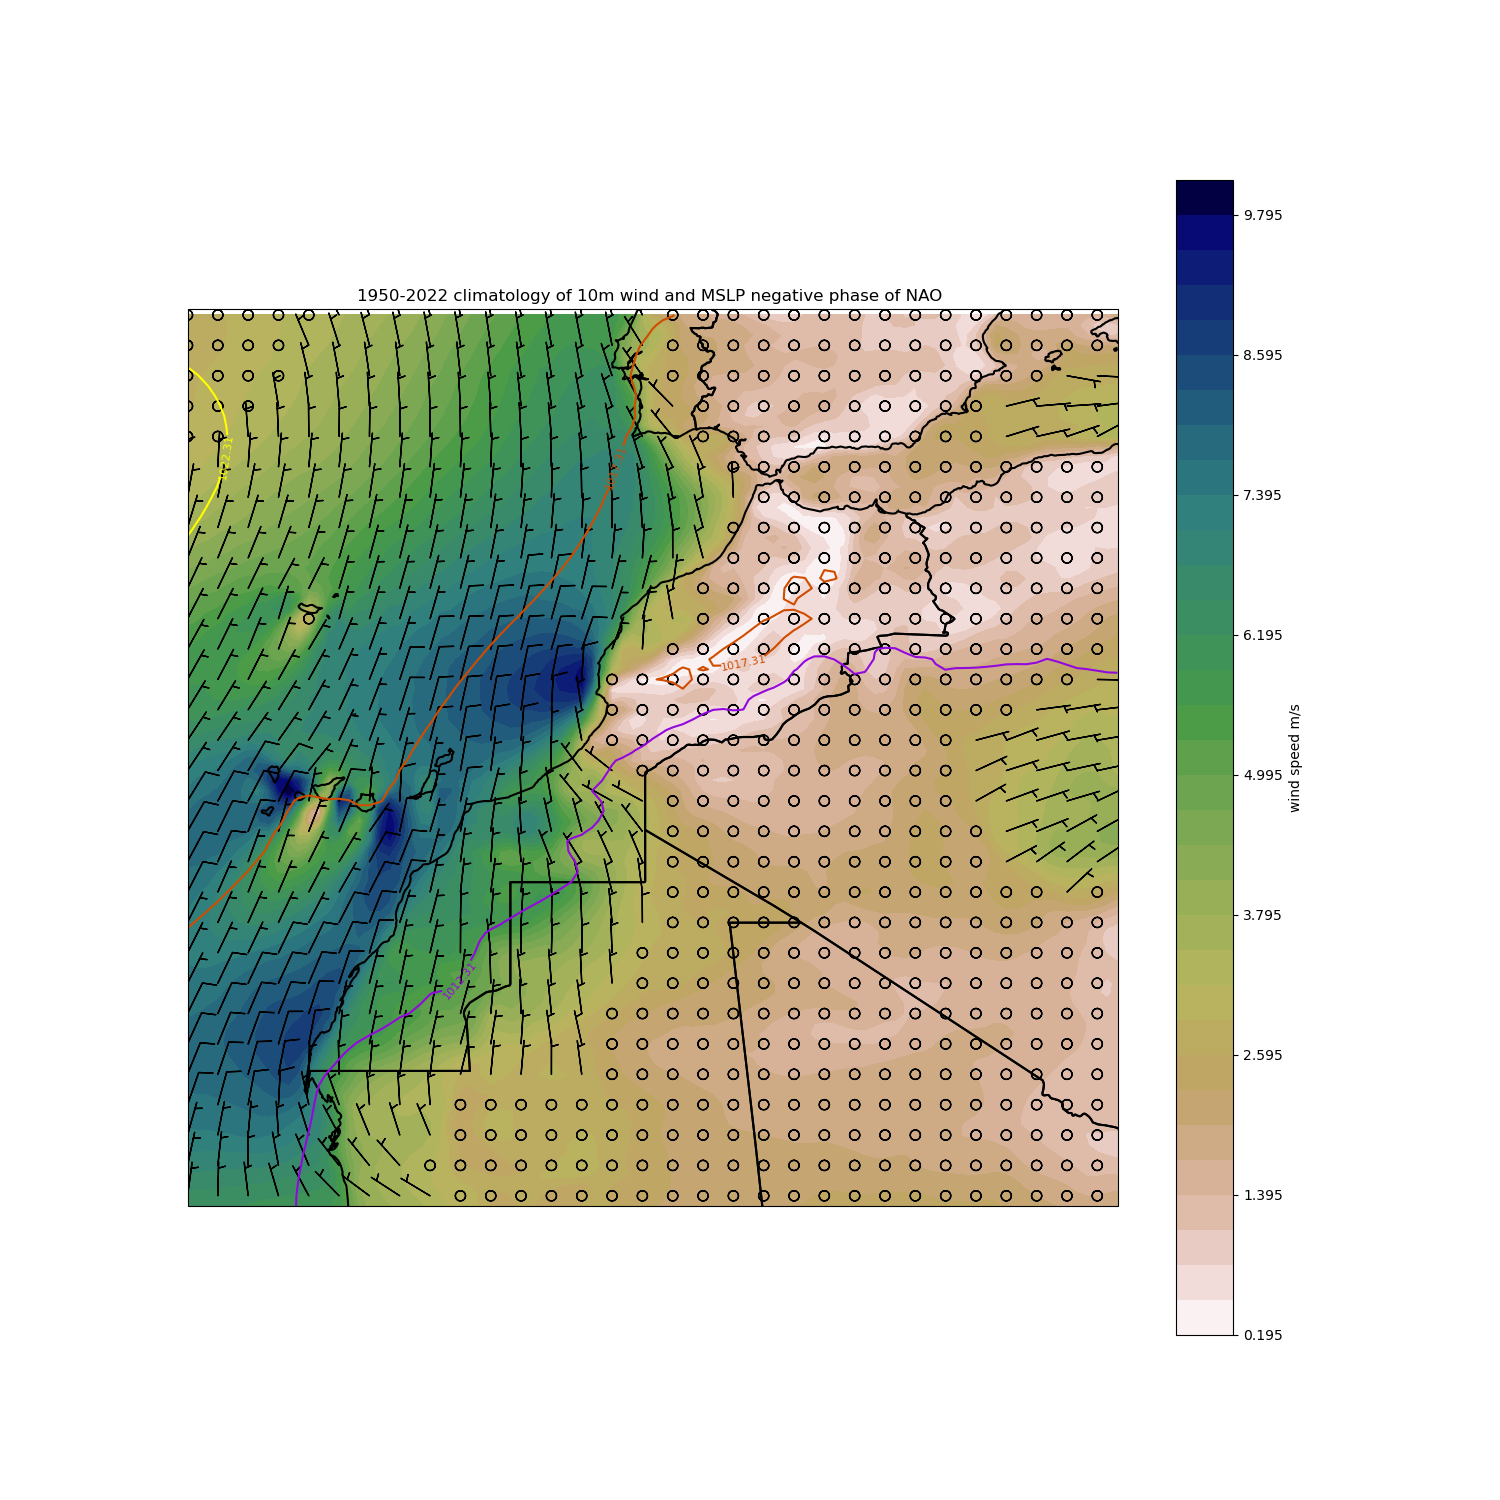
\includegraphics[scale=0.3]{NEG_PHASE.png}
\caption{Climatologie du vent et de la pression pour la phase NAO- (1950–2022).}
\label{fig:nao_negative}
\end{figure}

En revanche, la phase NAO- est caractérisée par des conditions favorables à l’upwelling :
\begin{itemize}
    \item \textbf{Direction du vent :} Les vents deviennent parallèles à la côte, favorisant un transport d'Ekman plus efficace. Cet alignement optimal est particulièrement marqué dans la région sud.
    \item \textbf{Intensité du vent :} Les vitesses moyennes atteignent environ 10 m/s, augmentant considérablement la dynamique de remontée des eaux froides.
    \item \textbf{Impact sur le CUI :} Une phase NAO- stimule fortement l’upwelling, renforçant la productivité biologique et soutenant les écosystèmes marins. Ces conditions sont idéales pour les activités de pêche dans la région.
\end{itemize}

\subsection{Discussion et implications}
Ces résultats démontrent que l'upwelling côtier au Maroc est influencé de manière significative par les phases de la NAO. La phase positive entraîne une diminution de l’upwelling, tandis que la phase négative l’intensifie. Ces variations impactent directement les écosystèmes marins et les activités économiques dépendantes, comme la pêche. Une analyse complémentaire, incluant des simulations climatiques futures, pourrait aider à anticiper les impacts du changement climatique sur cette dynamique essentielle.
